In questo primo esperimento si vuole studiare il comportamento di un convertitore di tensione switching - SMPC - di tipologia Buck ad \textbf{anello aperto}. Il circuito è rappresentato in Figura \ref{fig:Circuit1}. Sono stati utilizzati i seguenti componenti:
\begin{itemize}
    \item Circuito RLC:
    \subitem Resistenza di carico $R_L=50\Omega$, ottenuta dal parallelo di due resistenze da $100\Omega,1W$
    \subitem Induttore L, da scegliere tra i disponibili in lab.
    \subitem Condensatore C, da scegliere tra i disponibili in lab.
\end{itemize}
\begin{figure}[H]
    \centering
    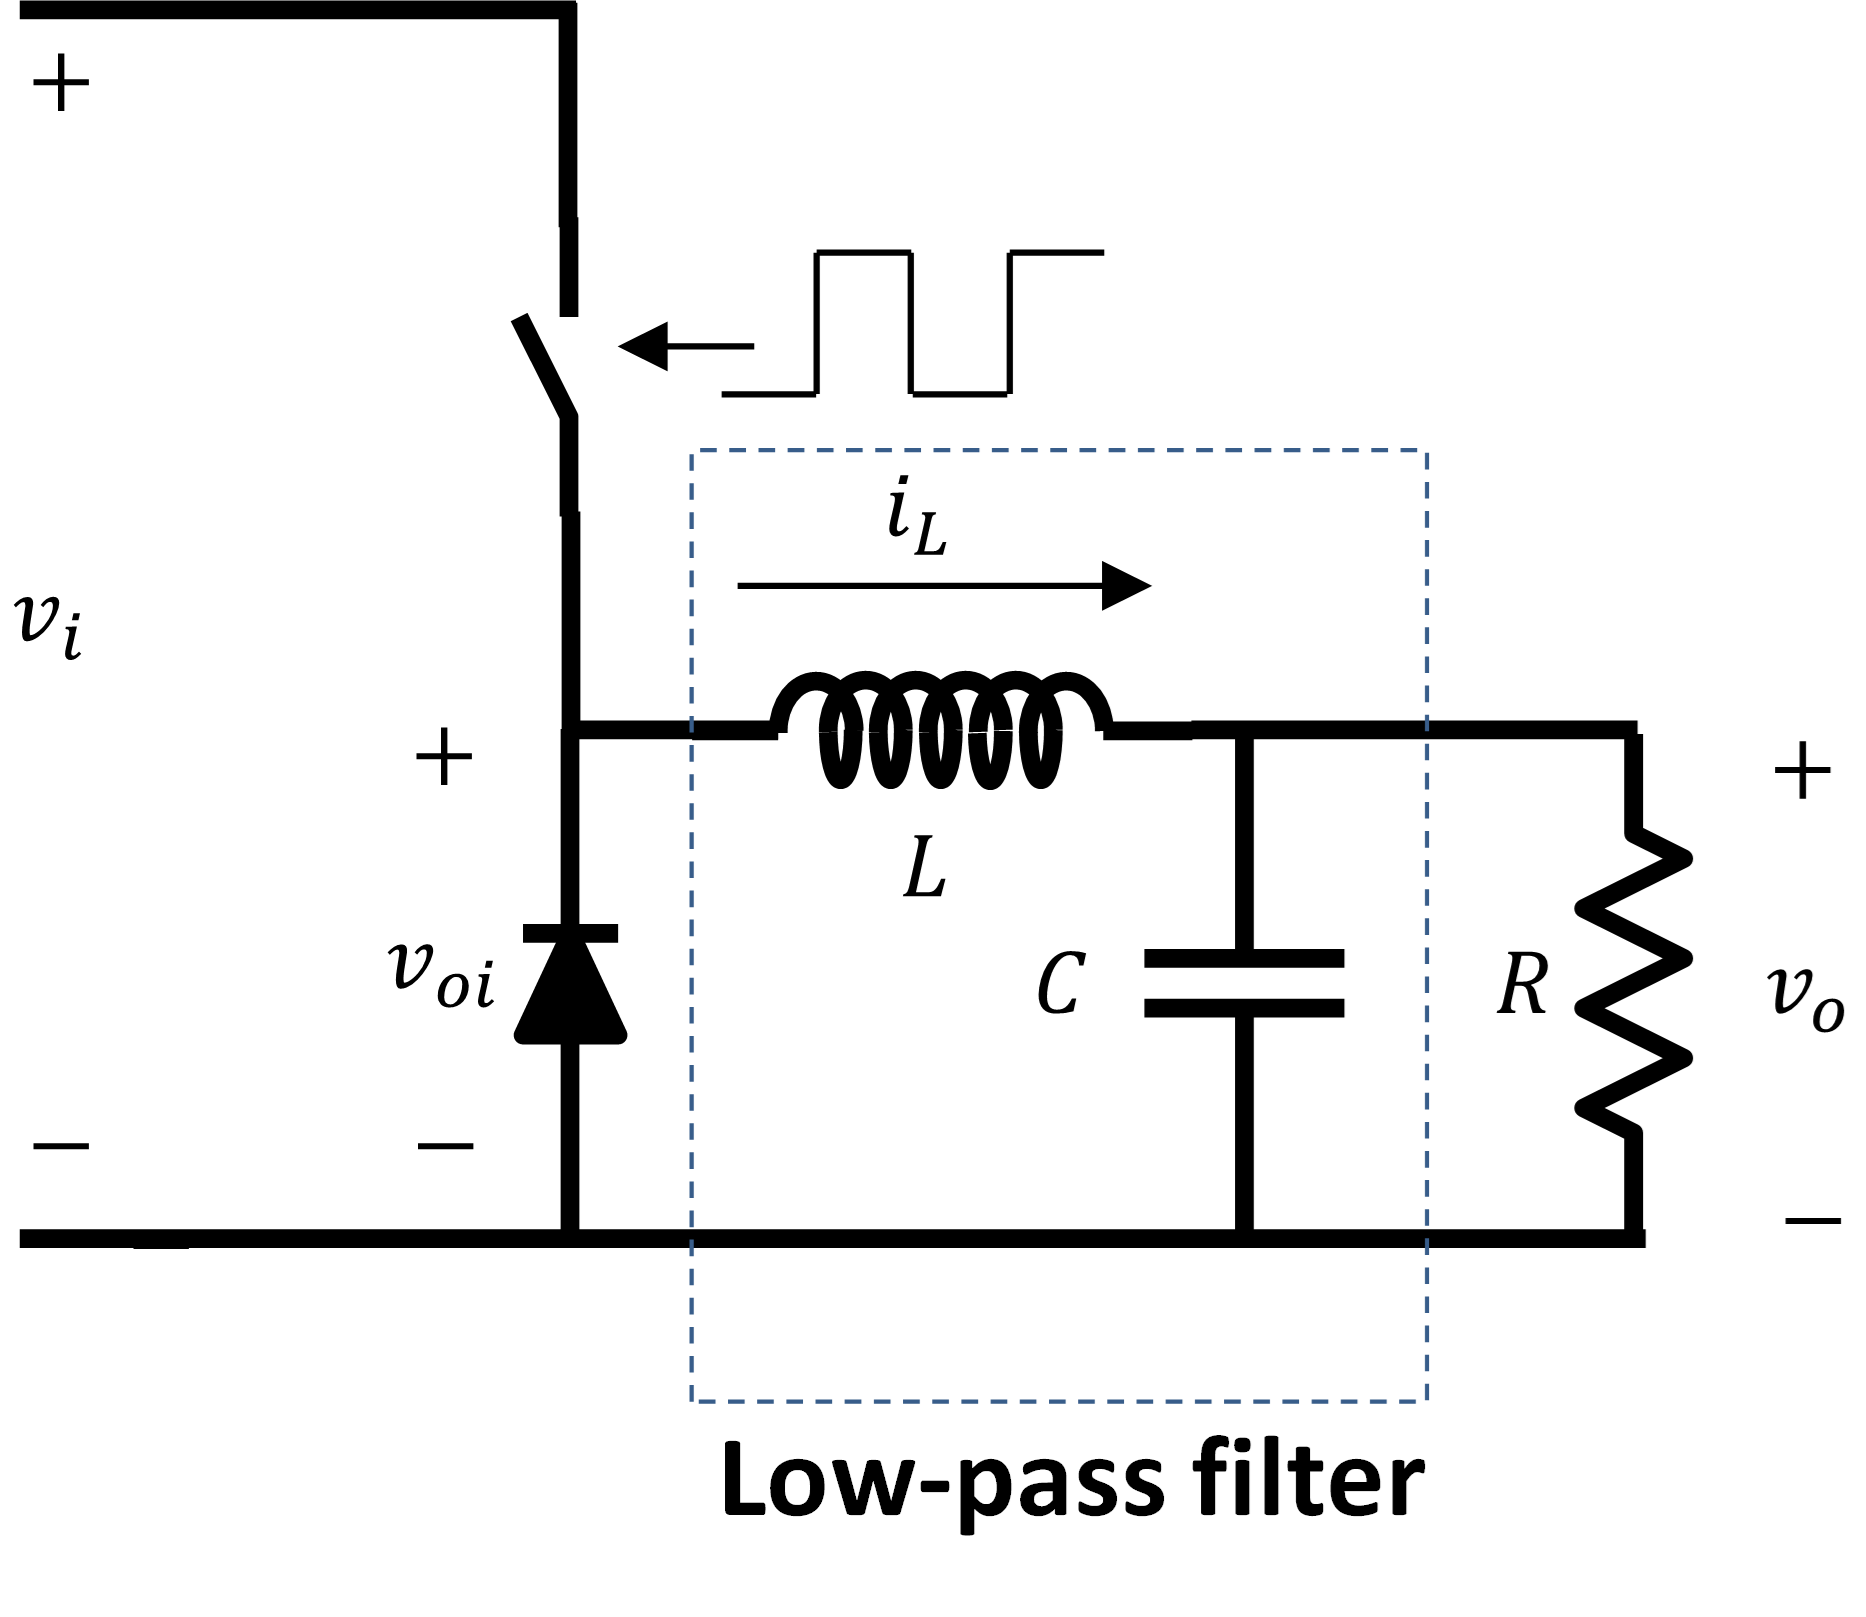
\includegraphics[width=0.5\linewidth]{images/Circuit1.png}
    \caption{Schema circuito}
    \label{fig:Circuit1}
\end{figure}
Il circuito è alimentato dalla tensione $Vi=+8V$.
\subsection{Dimensionamento di \textit{L} e \textit{C} - prelab}\label{ch:Cap1}
Consideriamo una frequenza di switching di $f=50kHz$ e una tensione di ingresso $V_i=+8V$. Determiniamo anzitutto il valore minimo dell'induttanza tale da garantire la condizione di \textit{continuos conduction mode} per un rate di duty cycle maggiore del 20\%. Vogliamo che sia quindi garantita
\begin{equation}
    I_{min}=V_O\left(\frac{1}{R}-\frac{1-\delta}{2L_{min}f}\right)=0\implies L_{min}=\frac{(1-\delta)R}{2f}=400\mu H
\end{equation}
Per cui scegliamo dagli induttori disponibili in laboratorio la seguente induttanza: $L=680\mu H$.\\\\
Dalla scelta di questa induttanza ci aspettiamo i seguenti valori per la minima e massima corrente di induzione
\begin{equation}
    I_{Lmax}=V_o\left(\frac{1}{R}+\frac{1-\delta}{2Lf}\right)=50.82mA
\end{equation}
\begin{equation}
    I_{Lmin}=V_o\left(\frac{1}{R}-\frac{1-\delta}{2Lf}\right)=13.18mA
\end{equation}
Determiniamo adesso un valore appropriato per il condensatore $C$ tale da garantire che l'output voltage ripple $\Delta V_c$ sia più piccolo di $100mV$. Partendo dalla relazione
\begin{equation}
    C=\frac{\Delta I_L}{8f\Delta V_c}\implies C=0.5881\mu F
\end{equation}
Ricaviamo abbiamo scelto il seguente valore per la capacità $C=1\mu F$.





\subsection{Assemblaggi e settaggi}
Dopo aver assemblato il circuito, seguendo lo schematico in Figura \ref{fig:Circuit1SPICE}. Abbiamo alimentato il circuito con il canale 2 dell'alimentatore da banco, in modo da avere la tensione di $V_i=+8V$ necessaria al funzionamento del circuito.
\begin{figure}[H]
    \centering
    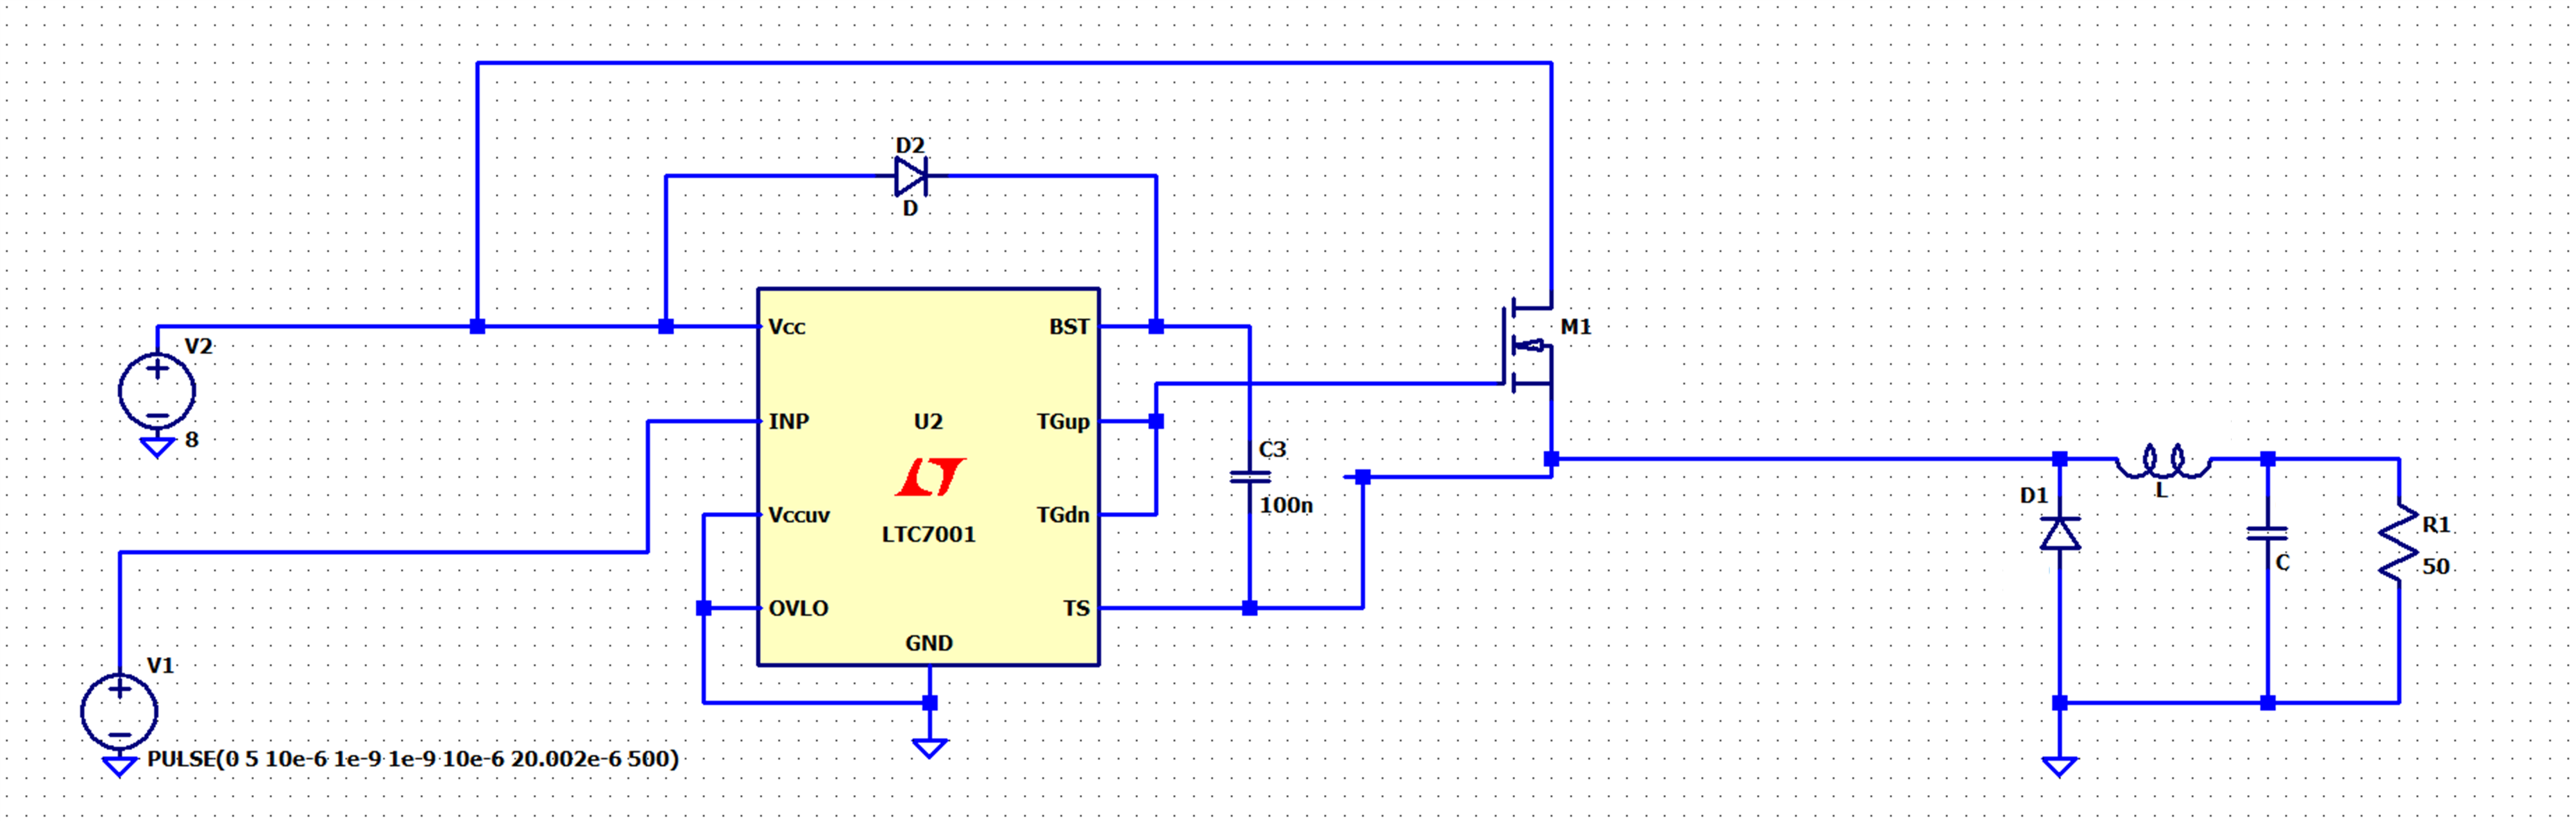
\includegraphics[width=\linewidth]{images/Circuit1SPICE.png}
    \caption{Schematico SPICE del circuito}
    \label{fig:Circuit1SPICE}
\end{figure}
Tramite il generatore di funzioni abbiamo fornito al terminale \textit{INP} dell' integrato LTC7001 il seguente segnale:
\begin{itemize}
    \item Forma d'onda: quadra
    \item Ampiezza: 5V picco-picco
    \item Tensione di offset: $V_{offset}=2.5V$
    \item Frequenza: $f=50kHz$
    \item Duty cycle: 50\%
\end{itemize}
\clearpage
\subsection{Risultati}
Riportiamo anzitutto tensioni al gate e al source del transistor, misurate tramite l'oscilloscopio e le relative schermate in Figura \ref{fig:GateMeasure1} e \ref{fig:SourceMeasure1}.
\begin{table}[H]
    \centering
    \begin{tabular}{|c|c|}
        \hline
        $Ampl(G)$&$17.3V$\\\hline
        $Ampl(S)$&$8.7V$\\\hline
    \end{tabular}
\end{table}
\begin{figure}[H]
    \centering
    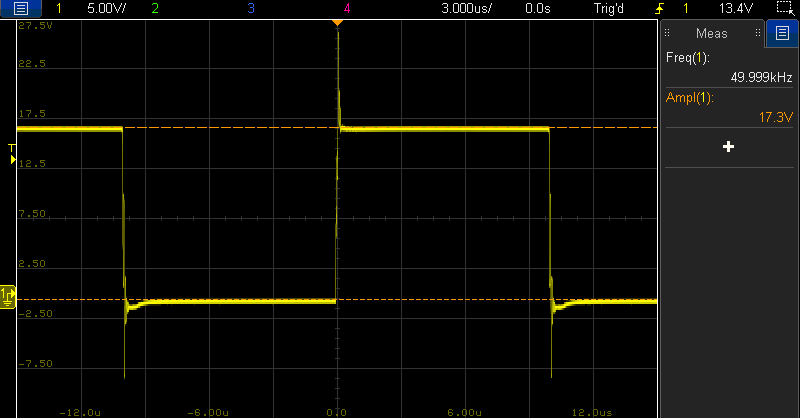
\includegraphics[width=0.6\linewidth]{images/scope_0.png}
    \caption{Segnale al gate del transistor}
    \label{fig:GateMeasure1}
\end{figure}
\begin{figure}[H]
    \centering
    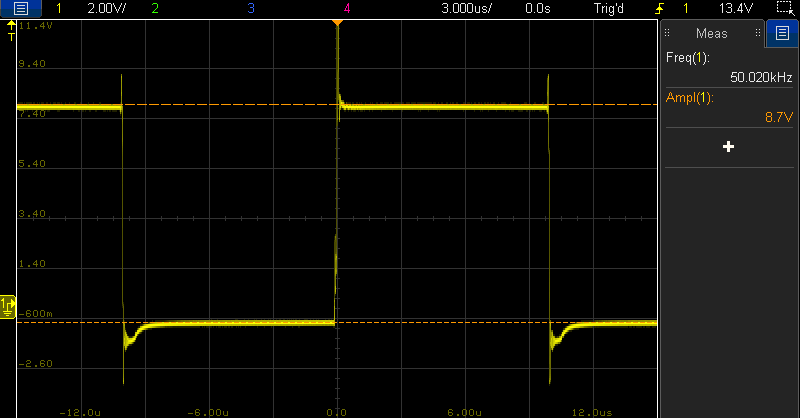
\includegraphics[width=0.6\linewidth]{images/scope_1.png}
    \caption{Segnale al source del transistor}
    \label{fig:SourceMeasure1}
\end{figure}
Misuriamo ora la tensione di uscita ai capi della resistenza di carico $R$ come funzione del tempo, riportiamo in Figura \ref{fig:OutputLoad1} la schermata dell'oscilloscopio
\begin{figure}[H]
    \centering
    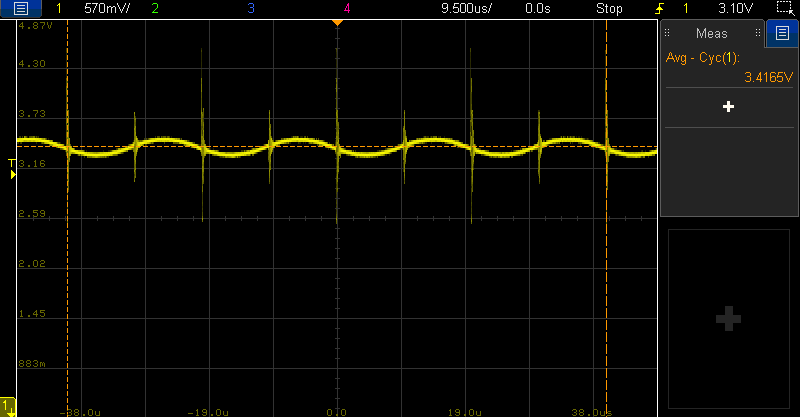
\includegraphics[width=0.6\linewidth]{images/scope_6.png}
    \caption{Tensione di uscita}
    \label{fig:OutputLoad1}
\end{figure}
Misuriamo anche il \textit{ripple} della tensione di uscita, sempre ai capi del carico $R$, riportiamo in Figura \ref{fig:OutputRipple1}  la schermata dell'oscilloscopio. Evidenziamo che la misura del voltage ripple è stata fatta impostando l'oscilloscopio in accoppiamento AC, in modo da eliminare le componenti continue del segnale di uscita.
\begin{figure}[H]
    \centering
    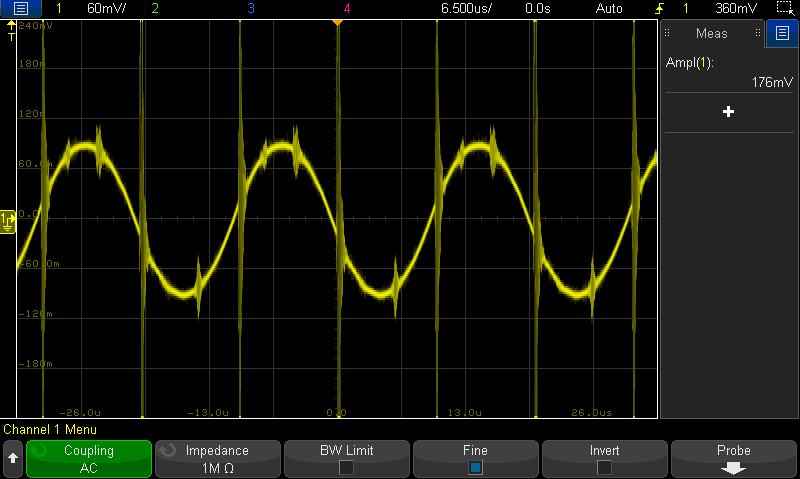
\includegraphics[width=0.6\linewidth]{images/scope_2.png}
    \caption{Apprezzamento del voltage ripple sul segnale di uscita}
    \label{fig:OutputRipple1}
\end{figure}
Notiamo dal grafico in Figura \ref{fig:OutputLoad1} che la media della tensione di uscita calcolata dall'oscilloscopio è di $3.4165V$ che si discosta dal valore atteso di $V_0=\delta V_i=4V$. Dal grafico in Figura \ref{fig:OutputRipple1} notiamo che il voltage ripple misurato è $176mV$ che è diverso dal valore di progetto ($100mV$). Entrambi queste anomalie sono dovute dapprima dalla configurazione a circuito aperto del circuito e in secondo luogo dalle incertezze i valori delle componenti. Notiamo inoltre che il segnale presenta notevole disturbo.
\clearpage


\subsubsection{Misura della corrente sull'induttore}
Usando una sonda di corrente il current probe (clamp it on one of the leads of the inductor), misuriamo ora la corrente che scorre nell'induttori durante pochi periodi di switching. Abbiamo riportato in Figura \ref{fig:CurrentInductor1} l'andamento della corrente misurato dall'oscilloscopio.
\begin{figure}[H]
    \centering
    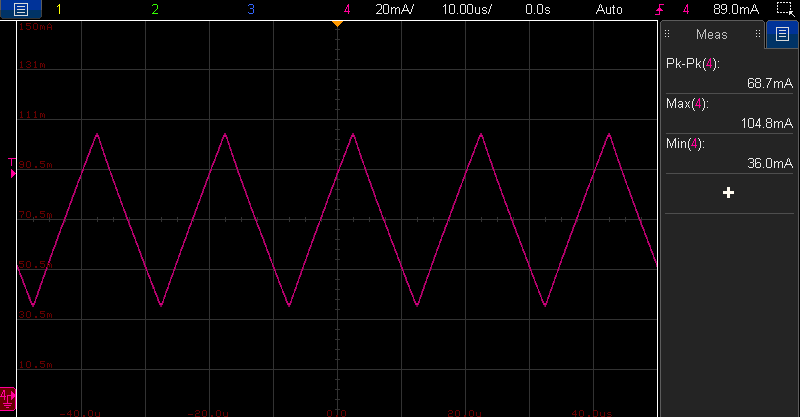
\includegraphics[width=0.8\linewidth]{images/scope_4.png}
    \caption{Corrente nell'induttore}
    \label{fig:CurrentInductor1}
\end{figure}
Riportiamo infine le misure delle correnti effettuate in modo da compararle con i valori teorici calcolati al punto \ref{ch:Cap1}
\begin{table}[H]
    \centering
    \begin{tabular}{|c|c|c|}
        \hline
        &Valore misurato&Valore teorico\\\hline\hline
        Corrente picco-picco&$68.7mA$&$37.64mA$\\\hline
        Corrente massima&$104.8mA$&$50.82mA$\\\hline
        Corrente minima&$36.0mA$&$13.18mA$\\\hline
    \end{tabular}
\end{table}
Notiamo anche qui un scostamento tra i valori teorici e i valori misurati. Per motivi già citati questi sono dovuti a incertezze nelle componenti e alla configurazione a circuito aperto.
\clearpage
\subsubsection{Dipendenza tensione di uscita - duty cycle}
Vogliamo in quest'ultimo punto valutare la dipendenza tra la tensione di uscita e il duty cycle. Abbiamo raccolto in laboratorio i dati presenti in Tabella \ref{tab:TabPlot}
\begin{table}[H]
    \centering
    \begin{tabular}{|c|c|}
        \hline
        Duty cycle (\%)&Output Voltage $V_o(V)$\\\hline\hline
        $20\%$&$1.0149V$\\\hline
        $30\%$&$1.8014V$\\\hline
        $40\%$&$2.6089V$\\\hline
        $50\%$&$3.4165V$\\\hline
        $60\%$&$4.2398V$\\\hline
        $70\%$&$5.0630V$\\\hline
        $80\%$&$5.2021V$\\\hline
    \end{tabular}
    \caption{Dati raccolti facendo variare il duty cycle del generatore}
    \label{tab:TabPlot}
\end{table}
Abbiamo infine plottato i risultati con MATLAB e prodotto il diagramma in Figura \ref{fig:MatlabPlot1}
\begin{figure}[H]
    \centering
    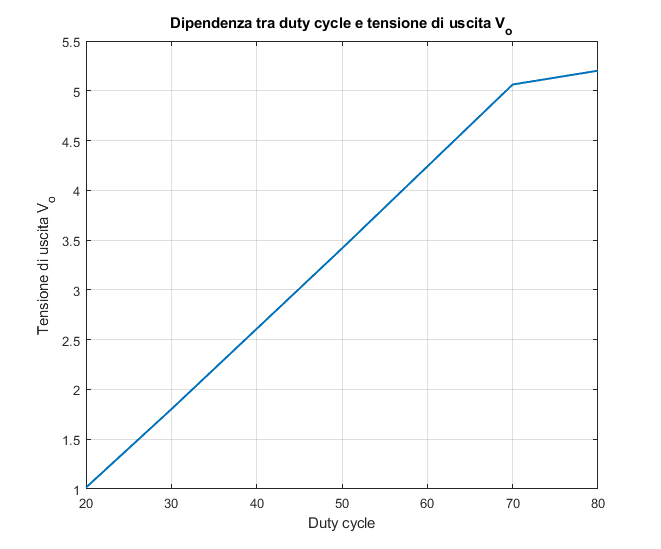
\includegraphics[width=0.7\linewidth]{images/Ris1TableDTCVo.png}
    \caption{Plot MATLAB dei dati raccolti in Tabella \ref{tab:TabPlot}}
    \label{fig:MatlabPlot1}
\end{figure}
Notiamo che l'andamento, a parte un piccolo scostamento nella misura con duty cycle 80\%, è lineare. Come dopotutto ci aspettiamo dalla relazione $V_o=\delta V_i$